\section{Construção manual de redes bayesianas}

\subsection{Primeira rede}
	A continuação se mostram as relações de dependencia para construir o grafo da rede bayesiana:
	\begin{itemize}
		\item age: marital-status
		\item marital-status: workclass
		\item workclass: hours-per-week,capital-gain,capital-loss
		\item hours-per-week: annual-income
		\item native-country: race,occupation
		\item race: workclass
		\item sex: relationship,hours-per-week
		\item relationship: marital-status
		\item occupation: capital-gain,capital-loss
		\item education-num: education
		\item education: occupation
		\item capital-gain: annual-income
		\item capital-loss: annual-income
		\item annual-income:
	\end{itemize}
	Cada linha é da forma $X_i : Childs( X_i )$ que representa todas as relações de causalidade que tem cada característica com algumas outras.\\
	De forma mais ilustrada, a Figura~\ref{fig:rede1} mostra a rede bayesiana construida com as linhas anteriores.
	\begin{figure}[ht]
		\centering
		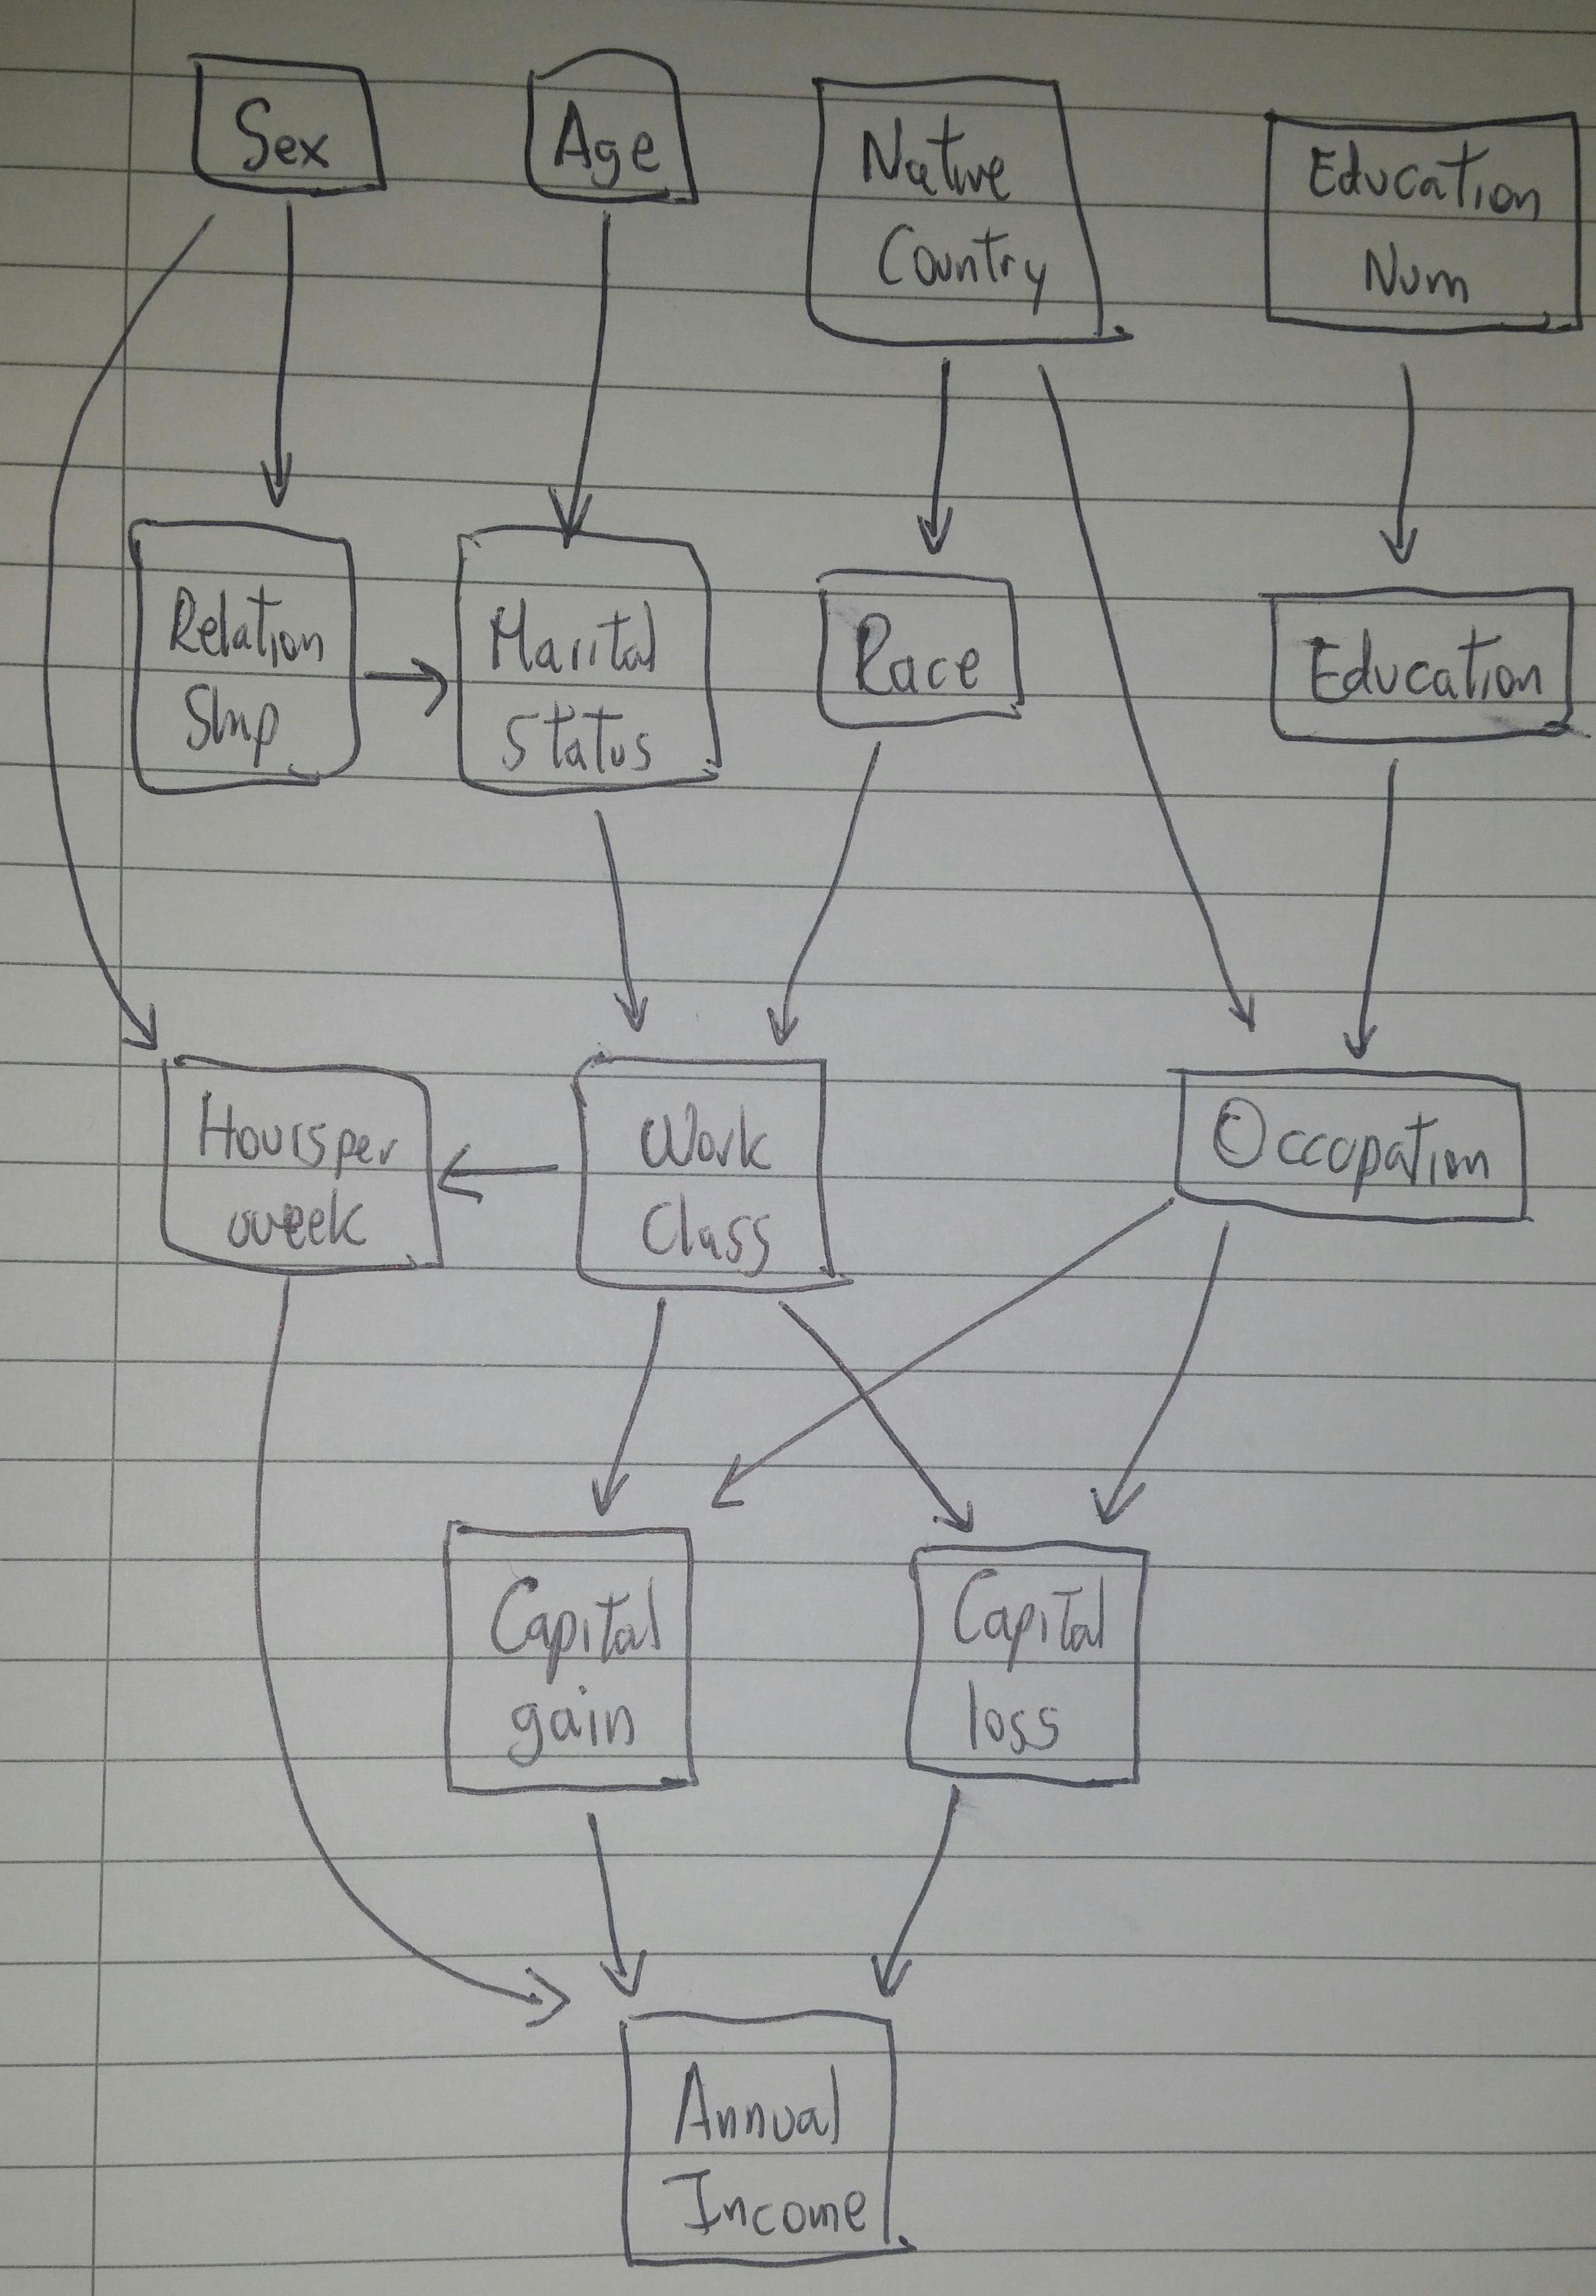
\includegraphics[height=12cm]{images/rede1}
		\caption{Primeira rede bayesiana}
		\label{fig:rede1}
	\end{figure}
	\\
	Para construir esta rede se levou em consideração as seguintes suposições:
	\begin{itemize}
		\item Sexo, idade e pais de origem não tem como causa alguma das outras características porque na vida real não dependem de nada
		\item O pais de origem da pessoa influi na raza, por exemplo é mais seguro que uma pessoa com rasgos asiáticos tenha um pais de origem asiático
		\item O pais de origem influi na ocupação da pessoa porque não existem todas as ocupações em todos os países do mundo (e.g. astronauta)
		\item O estado civil e a raza da pessoa influem no tipo de trabalho que tem (e.g. pessoas casadas podem ter trabalhos privados)
		\item O tipo de trabalho e o sexo influem nas horas de trabalho por semana porque existem trabalhos só para mulheres que não precisam muitas horas
		\item O tipo de trabalho e a ocupação influem nos ganhos e perdas de capital diretamente (e.g. algumas ocupações ganham mais dinheiro que outras em alguns casos, dependendo do tipo de trabalho)
		\item Para os ingresos anuales da pessoa, temos em consideração os ganhos, perdas de capital e as horas de trabalho semanais (e.g. uma pessoa que perde muito, tem poucos ingresos anuais, da mesma forma para alguém que ganha muito)
	\end{itemize}
	
\subsection{Segunda rede}
	Da mesma forma que para a anterior rede temos:
	\begin{itemize}
		\item age: marital-status
		\item marital-status: workclass
		\item workclass: relationship,hours-per-week
		\item hours-per-week: capital-gain,capital-loss
		\item native-country: occupation,education,education-num,race
		\item race: education
		\item sex: workclass
		\item relationship: capital-gain,capital-loss
		\item occupation: capital-gain,capital-loss
		\item education-num: education
		\item education: marital-status
		\item capital-gain: annual-income
		\item capital-loss: annual-income
		\item annual-income:
	\end{itemize}
	A Figura~\ref{fig:rede2} mostra todas as relações de dependencia que tem cada característica.
	\begin{figure}[ht]
		\centering
		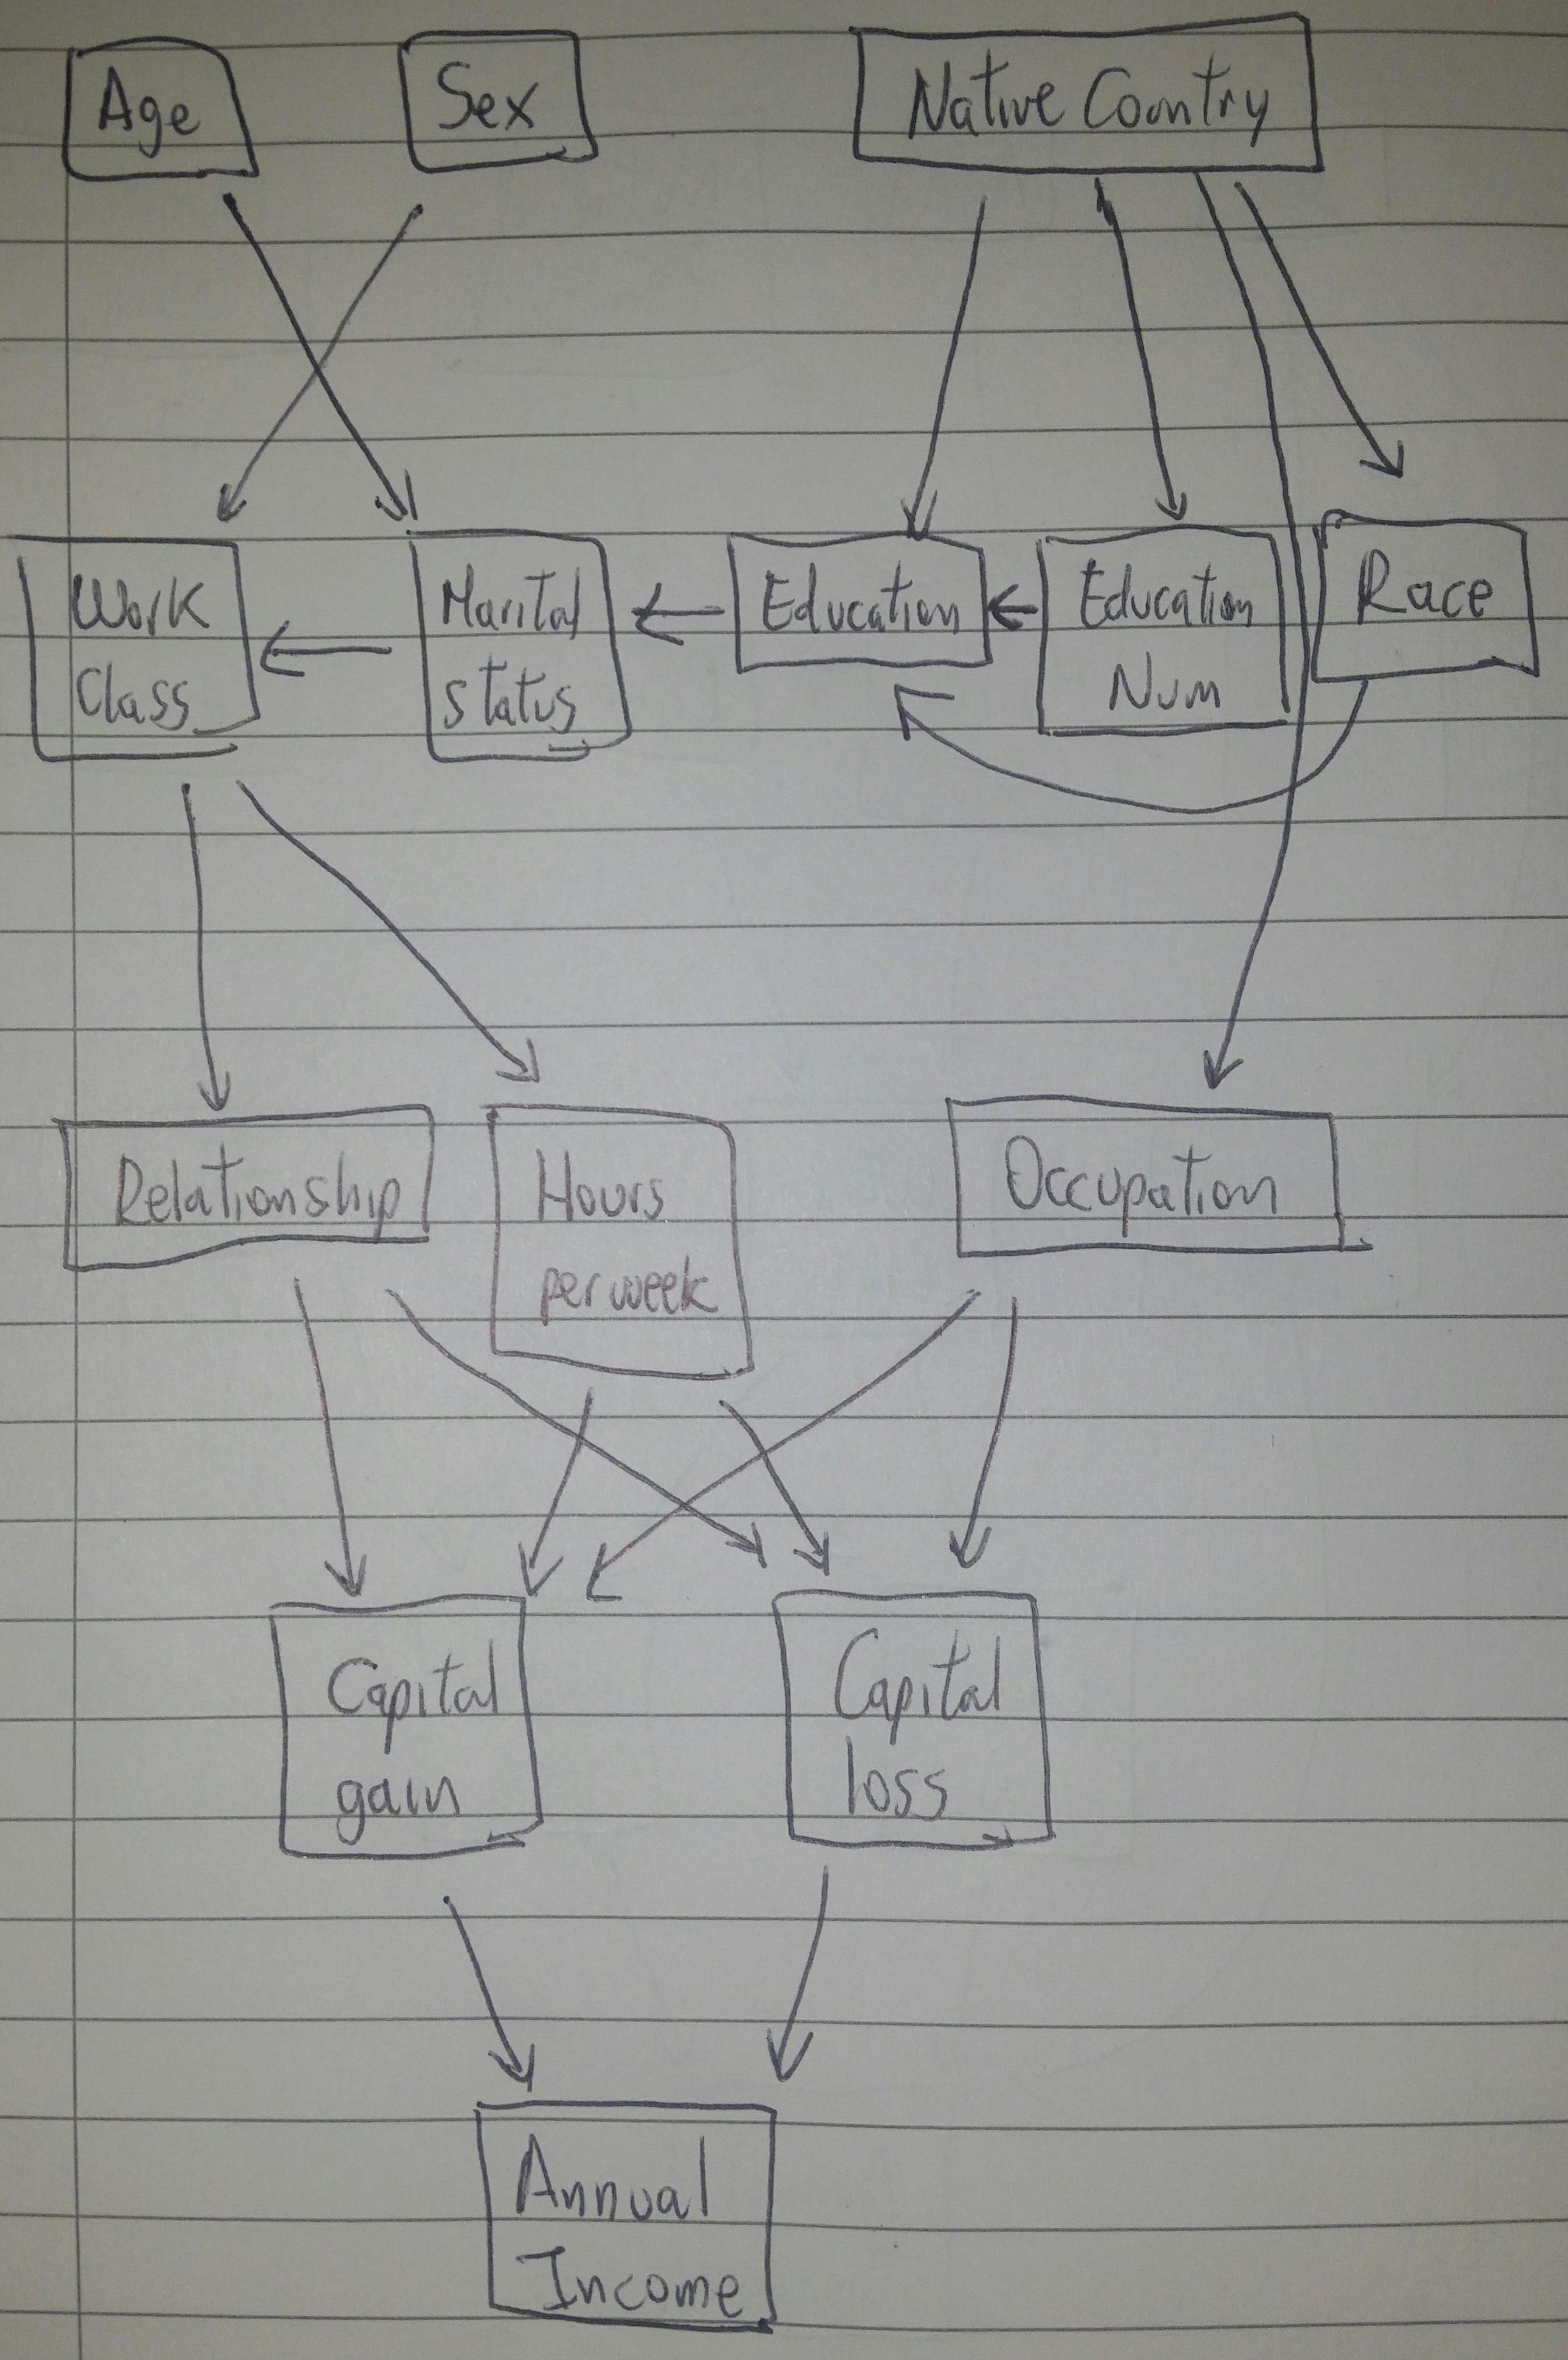
\includegraphics[height=12cm]{images/rede2}
		\caption{Segunda rede bayesiana}
		\label{fig:rede2}
	\end{figure}
	\\
	Tendo en consideração as seguintes suposições podemos construir esta rede:
	\begin{itemize}
		\item A educação, raza e a ocupação dependem do pais de origem da pessoa por as oportunidades que podem existir li
		\item O estado civil depende da idade e a educação que tem a pessoa (e.g. não muitos jovens se casam, gente que consegue nível universitario se casa)
		\item A educação depende da raza da pessoa em alguns lugares do mundo (com muito racismo)
		\item O sexo e o estado civil influi no tipo de trabalho pela mesma razão da rede anterior
		\item Dependendo o tipo de trabalho pode necessitar mais horas de trabalho e também influi no tipo de relação que a pessoa tem (e.g. solteiro, casado)
		\item Os ganhos e perdas de capital dependem das horas trabalhadas na semana porque mais horas trabalhadas podem significar mais ganhos
		\item Da mesma forma, uma melhor ocupação pode ganhar o perder mais que outras
		\item A relação também influi porque se gasta mais quando a pessoa está uma relação
		\item Os ingresos anuais dependem de quanto a pessoa ganha e perde capital
	\end{itemize}

\subsection{Terceira rede}
	Por último, a terceira rede construída manualmente é:
	\begin{itemize}
		\item age: capital-gain,capital-loss
		\item marital-status: workclass
		\item workclass: hours-per-week
		\item hours-per-week: annual-income
		\item native-country: race,capital-gain,capital-loss
		\item race: relationship
		\item sex: capital-gain,capital-loss
		\item relationship: marital-status
		\item occupation: workclass
		\item education-num: workclass
		\item education: workclass
		\item capital-gain: education,education-num
		\item capital-loss: education,education-num
		\item annual-income:
	\end{itemize}
	
	Na Figura~\ref{fig:rede3} a continuação mostra a última rede bayesiana construída manualmente.
	\begin{figure}[ht]
		\centering
		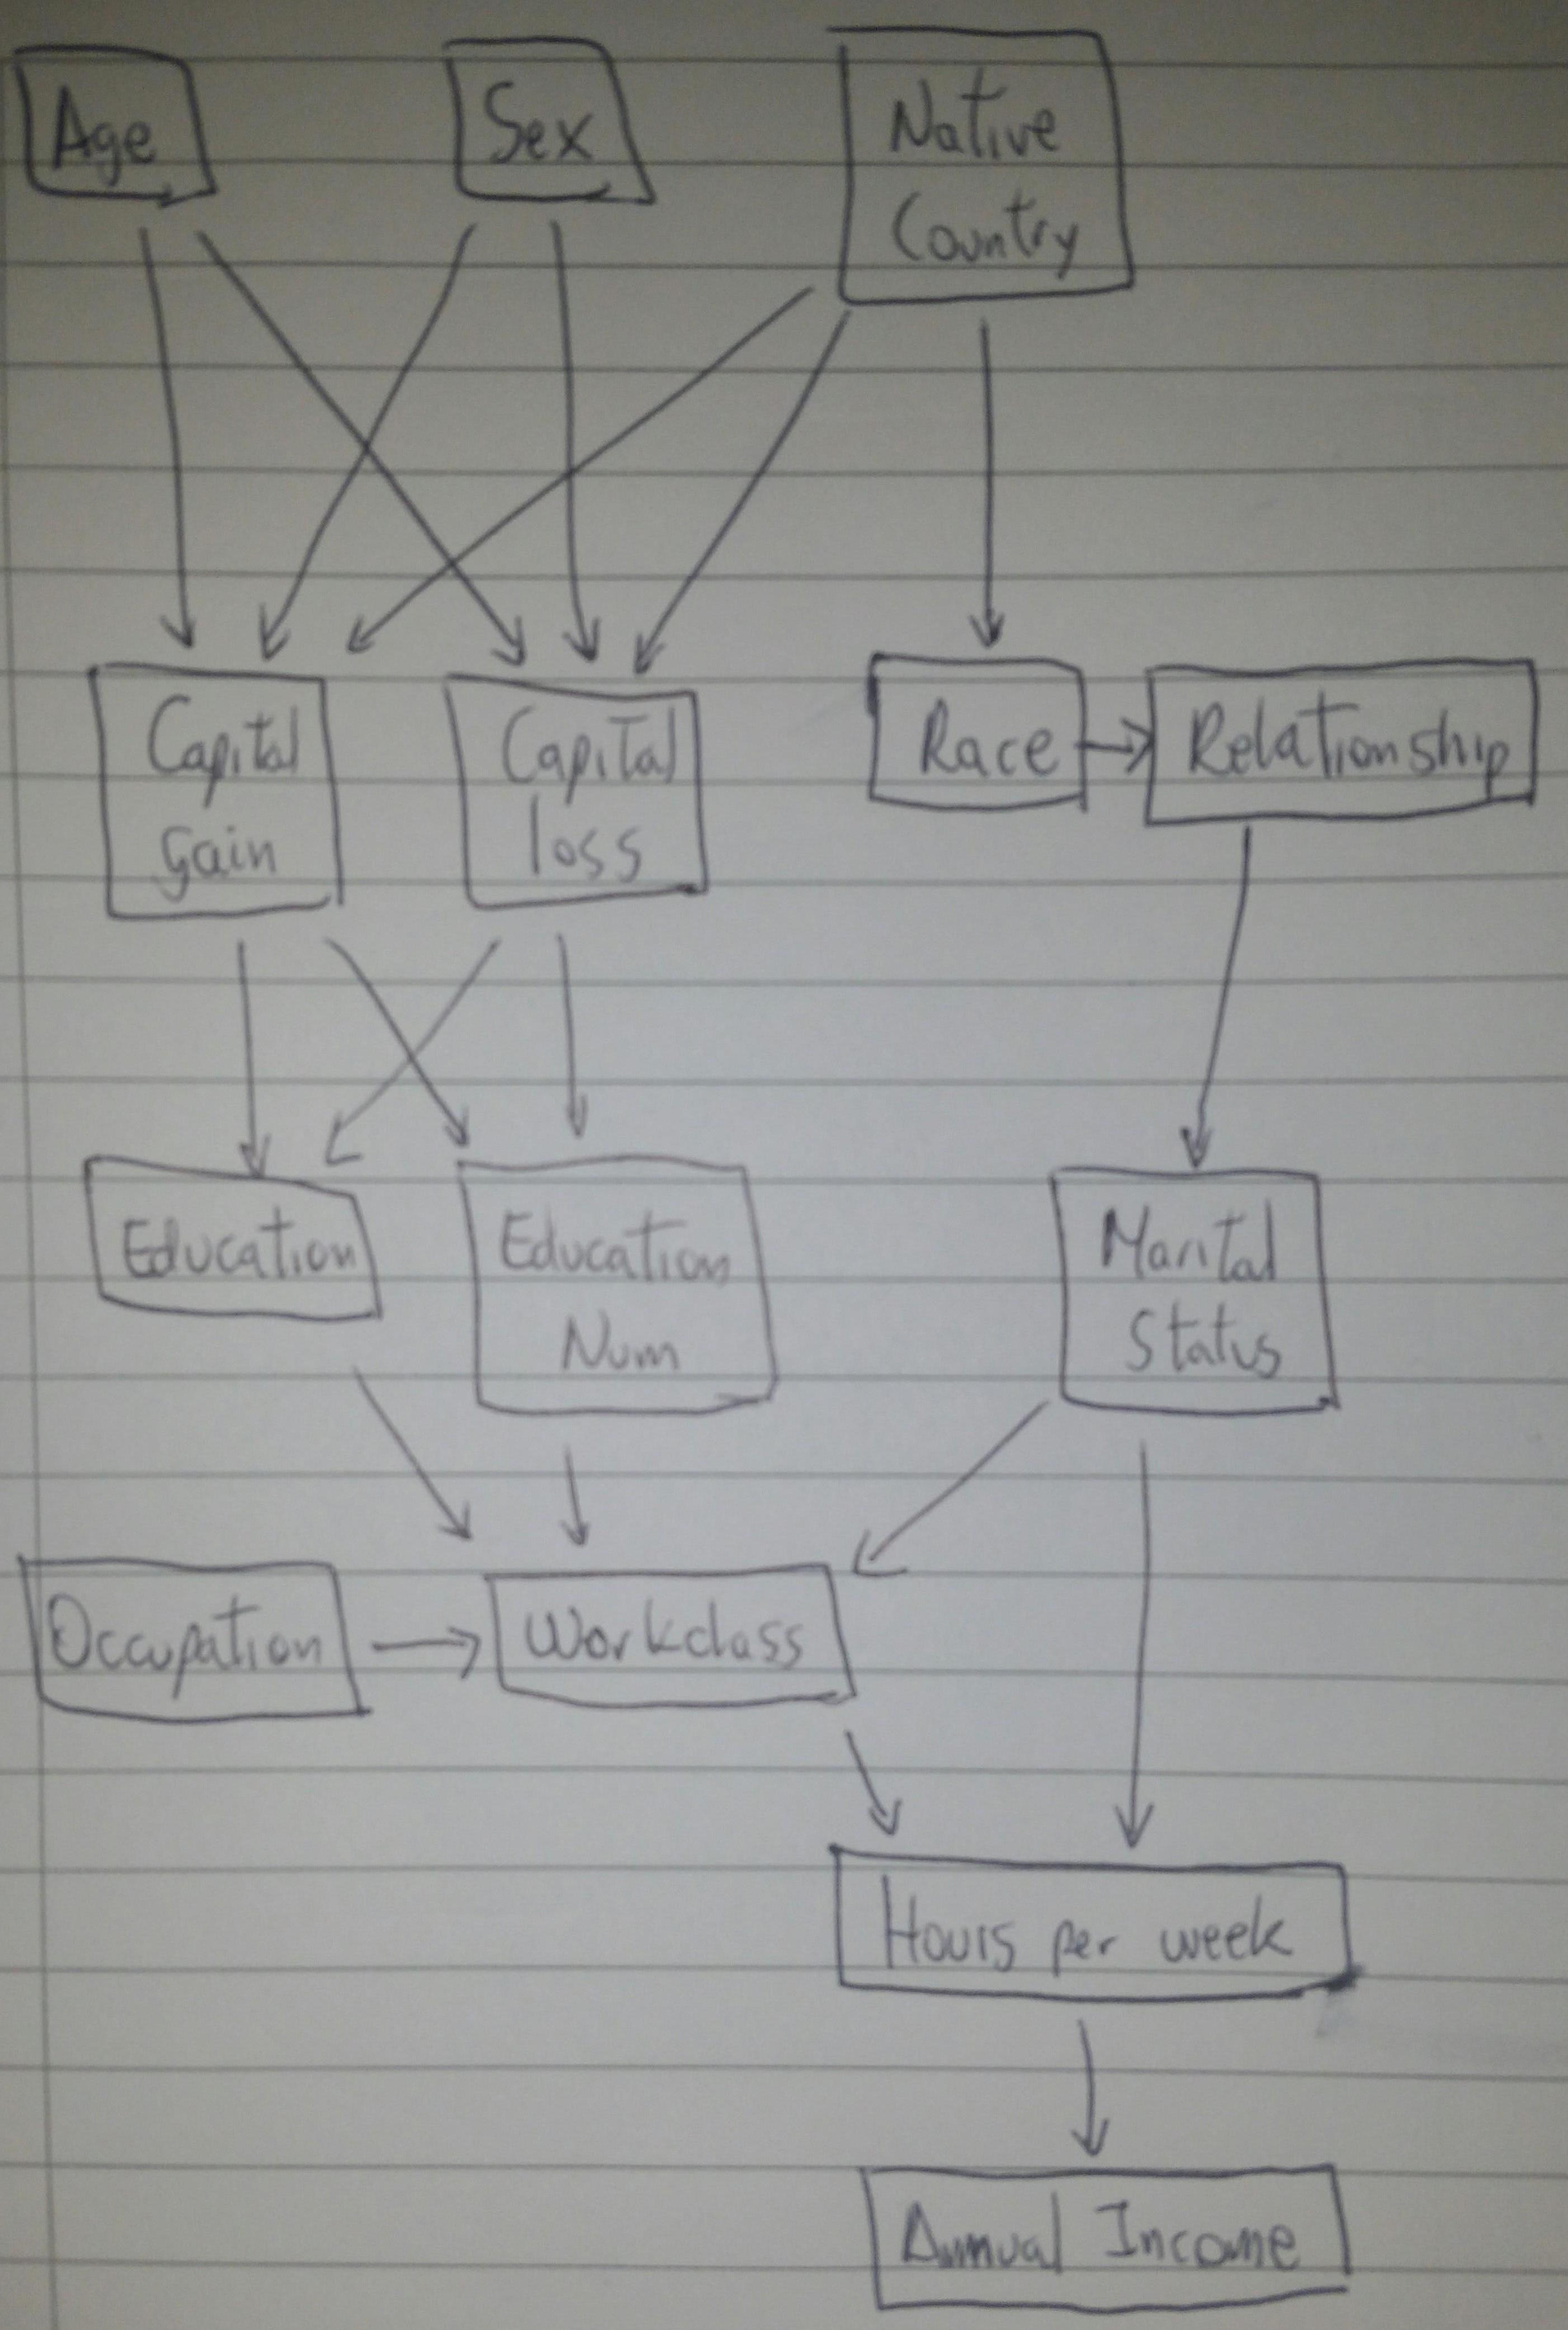
\includegraphics[height=12cm]{images/rede3}
		\caption{Terceira rede bayesiana}
		\label{fig:rede3}
	\end{figure}
	\\
	Para esta última rede se levou em consideração o seguinte:
	\begin{itemize}
		\item A idade, o sexo e o pais de origem influem nos ganhos e perdas de capital porque uma pessoa mais joven não tem muitas perdas, uma mulher pode ter muitas perdas por muitas compras e o pais de origem pode ter uma crise que gere muitas perdas as pessoas.
		\item Dependendo dos ganhos e perdas de capital da pessoa pode conseguir um nível de educação maior
		\item O tipo de trabalho é afeitado pela educação, o estado civil e a ocupação porque, por exemplo, algumas ocupações não são comumente trabalhadas de forma privada
		\item A ocupação da pessoa não depende de nada porque pode trabalhar em qualquer coisa que ele quizer
		\item As horas de trabalho semanais tem que ver com o estado civil (e.g. pessoas casadas trabalham mais que as solteiras) e o tipo de trabalho (e.g. trabalhos privados o independentes não tem um cronograma feito)
		\item Os ingresos anuais só dependem das horas trabalhadas semanalmente (e.g. se trabalha mais horas, pode ganhar mais)
	\end{itemize}
	
\clearpage